\documentclass{article}
\usepackage{include/nips13submit_e,times}
%%%%%%%%%%%%%%%%%%%%%%%%%%%%%%%%%%%%%%%%%%%%%%%%%%%%%%%%%%%
%%%% EDITING HELPER FUNCTIONS  %%%%%%%%%%%%%%%%%%%%%%%%%%%
%%%%%%%%%%%%%%%%%%%%%%%%%%%%%%%%%%%%%%%%%%%%%%%%%%%%%%%%%%

%% NA: needs attention (rough writing whose correctness needs to be verified)
%% TBD: instructions for how to fix a gap ("Describe the propagation by ...")
%% PROBLEM: bug or missing crucial bit 

%% use \fXXX versions of these macros to put additional explanation into a footnote.  
%% The idea is that we don't want to interrupt the flow of the paper or make it 
%% impossible to read because there are a bunch of comments.

%% NA's (and TBDs, those less crucially) should be written so 
%% that they flow with the text.

\definecolor{WowColor}{rgb}{.75,0,.75}
\definecolor{SubtleColor}{rgb}{0,0,.50}

% inline
\newcommand{\NA}[1]{\textcolor{SubtleColor}{ {\tiny \bf ($\star$)} #1}}
\newcommand{\LATER}[1]{\textcolor{SubtleColor}{ {\tiny \bf ($\dagger$)} #1}}
\newcommand{\TBD}[1]{\textcolor{SubtleColor}{ {\tiny \bf (!)} #1}}
\newcommand{\PROBLEM}[1]{\textcolor{WowColor}{ {\bf (!!)} {\bf #1}}}

% as margin notes

\newcounter{margincounter}
\newcommand{\displaycounter}{{\arabic{margincounter}}}
\newcommand{\incdisplaycounter}{{\stepcounter{margincounter}\arabic{margincounter}}}

\newcommand{\fTBD}[1]{\textcolor{SubtleColor}{$\,^{(\incdisplaycounter)}$}\marginpar{\tiny\textcolor{SubtleColor}{ {\tiny $(\displaycounter)$} #1}}}

\newcommand{\fPROBLEM}[1]{\textcolor{WowColor}{$\,^{((\incdisplaycounter))}$}\marginpar{\tiny\textcolor{WowColor}{ {\bf $\mathbf{((\displaycounter))}$} {\bf #1}}}}

\newcommand{\fLATER}[1]{\textcolor{SubtleColor}{$\,^{(\incdisplaycounter\dagger)}$}\marginpar{\tiny\textcolor{SubtleColor}{ {\tiny $(\displaycounter\dagger)$} #1}}}

\usepackage{include/preamble}
\usepackage{natbib}
\usepackage{tikz}
\usetikzlibrary{arrows}

\title{Non-degenerate Priors for Arbitrarily Deep Networks}


\author{
David Duvenaud \\
University of Cambridge \\
\texttt{dkd23@cam.ac.uk} \\
\And
Oren Rippel \\
Harvard University \\
\texttt{rippel@math.mit.edu} \\
\AND
Ryan Adams \\
Harvard University \\
\texttt{rpa@seas.harvard.edu} \\
\And
Zoubin Ghahramani \\
University of Cambridge \\
\texttt{zoubin@eng.cam.ac.uk} \\
}


% Custom notation
\newcommand{\fdeep}{f^{1:L}}
\newcommand{\flast}{f^{L}}
\newcommand{\Jx}{J_{\vx \rightarrow \vy}}
\newcommand{\Jxx}{J_{\vx \rightarrow \vy}(\vx)}
\newcommand{\Jy}{J_{\vy \rightarrow \vx}}
\newcommand{\Jyy}{J_{\vy \rightarrow \vx}(\vy)}
\newcommand{\detJyy}{ \left| J_{\vy \rightarrow \vx}(\vy) \right|}


% The \author macro works with any number of authors. There are two commands
% used to separate the names and addresses of multiple authors: \And and \AND.
%
% Using \And between authors leaves it to \LaTeX{} to determine where to break
% the lines. Using \AND forces a linebreak at that point. So, if \LaTeX{}
% puts 3 of 4 authors names on the first line, and the last on the second
% line, try using \AND instead of \And before the third author name.

\newcommand{\fix}{\marginpar{FIX}}
\newcommand{\new}{\marginpar{NEW}}

\nipsfinalcopy % Uncomment for camera-ready version

\begin{document}


\maketitle

\begin{abstract}
%We first demonstrate a pathology of typical deep architectures: as the number of layers increase, latent representations 
Choosing approrpriate architectures and initialization strategies are crucial to good performance of deep networks.  To shed light on this problem, we analyze the analogous problem of constructing useful priors on deep functions.
%A good latent representation captures all the relevant degrees of freedom of the manifold on which the data lie.  
We show that for typical deep architectures, the representational capacity of the network tends to capture fewer degrees of freedom as the number of layers increases, retaining only a single degree of freedom in the limit.  
%In addition, gradient-based learning becomes intractable.  
We propose alternate priors on network structure which do not suffer from these pathologies. %:  First, simply connecting the input layer to every other layer.  Second, a more general prior of computation graphs based on the Aldous-Hoover graph representation.  
We also derive novel kernels obtained by composing infinitely-many feature transforms.
\end{abstract}

\section{Introduction}

Much recent work on deep networks has focused on weight initialization \cite{martens2010deep}, regularization \cite{lee2007sparse} and network architecture \cite{poon2011sum}.  The interactions between these different design decisions can be complex and difficult to characterize.  We propose to approach the design of deep architectures by examining the problem of creating priors on functions with desirable properties.  Although inference in fully Bayesian models is generally difficult, well-defined priors allow us to characterize models in a data-independent way.  Once we identify classes of priors with useful properties, these models may suggest regularization, initialization, and architecture choices with similar properties.

In this paper, we examine a simple and flexible class of priors on functions, Gaussian processes (\gp{}s), and their extension into a deep architecture: Deep \gp{}s \cite{damianou2012deep}.  Deep \gp{}s are simply a prior on compositions of functions, each of which is distributed independently according to a \gp{} prior:
%
\begin{align}
f^{1:L}(\vx) = f^L(f^{L-1}(\dots f^3(f^2(f^1(\vx)))\dots)) \qquad \textnormal{ where each $f^\ell \simiid \GPt{0}{k(\vx, \vx')}$}
\end{align}

Although inference in these models is non-trivial, they can be derived as a special case of multi-layer perceptrons (MLPs), and so are a good candidate for a generative model of functions with similar properties to existing neural networks.

%Section \ref{sec:relating} will derive the precise relationship between deep \gp{}s and MLPs.  Section \ref{sec:1d} will examine the asymptotic behavior of arbitrarily deep one-dimensional \gp{}s.  Section \ref{sec:theorem} gives a theorem characterizing the Jacobian of a deep multidimensinal \gp{}.  Section 
%Deep networks have become an important tool for machine learning [cite].  However, training these models are difficult, Many arguments have been made for the need for deep architectures [cite Bengio].  However, it is hard to know what effect the deepness of an architecture has.  Also, the weights don't necessarily move that much from their initialization.

%Good initialization schemes can help, but we are interested in creating distributions on deep functions so that most of the mass is on functions without any pathologies.  Also, we might be able to show that the pathologies we show that most functions exhibit means that it will be hard to learn them by gradient descent.





\section{Relating deep nets and deep Gaussian processes}
\label{sec:relating}
%There are two ways to view deep Gaussian processes as neural networks.  First, we can
%We introduce a generative non-parametric model to address this problem.  Our approach is based on the GP-LVM ~\cite{lawrence2004gaussian,salzmann2008local,lawrence2009non}, a flexible nonparametric density model.  

%\cite{NIPS2005_424} showed that kernel machines such as \gp{}s have limited generalization ability when they are forced to use a 'local' kernel.

%\subsection{A neural net with one hidden layer}

In the typical definition of a multi-layer perception, the hidden units of the first layer are defined as:
%
\begin{align}
\Phi(\vx) = h^{(1)}(\vx) = \sigma( b^{(1)} + W^{(1)}\vx )
\end{align}
%
where $h$ are the hidden unit activations, $b$ is a bias vector and $W$ is a weight matrix. The output vector $f(\vx)$ is simply a weighted sum of these hidden unit activations:
%
\begin{align}
f(\vx) = V \sigma \left( b^{(n)} + W^{(1)} h(\vx) \right)  = V h(\vx) 
\end{align}
%
where $V$ is another weight matrix.

There exists a simple correspondence between one-layer MLPs and \gp{}s \cite{neal1995bayesian}.  \gp{} priors can be viewed as the limiting distribution of a neural network with infinitely many hidden units.  More precisely, for any model of the form
%
\begin{align}
f(x) = \frac{1}{K}{\mathbf \alpha}\tra \Phi(x) = \frac{1}{K} \sum_{i=i}^K \alpha_i \phi_i(x),
\label{eq:one-layer-nn}
\end{align}
%
with fixed feature vector $\Phi(x)$ and i.i.d. $\alpha$'s with zero mean and finite variance $\sigma^2$, the central limit theorem implies that as $K \rightarrow \infty$, any two function values $f(x), f(x')$ have a joint distribution approaching $\Nt{0}{\frac{\sigma^2}{K}\sum_{i=1}^K \phi_i(x)\phi_i(x')}$.  The result is surprisingly general:  It doesn't put any constraints on what the features are (other than having bounded activation), nor does it require that the feature weighs $\alpha$ be Gaussian distributed.  

We can also work backwards to derive a one-layer MLP from a \gp{}:  Mercer's theorem implies that any positive-definite kernel function corresponds to an inner product of features: $k(x, x') = \Phi(x) \tra \Phi(x)$.
%
Thus in the one layer case, the correspondence between MLPs and \gp{}s is simple:  The features $\phi(\vx)$ of the \gp{} correspond to the hidden units of the MLP.


\subsection{Multiple hidden layers}

\begin{figure}
\def\layersep{1.14cm}
\def\nodesep{.75cm}
\def\nodesize{.35cm}

\newcommand{\numdims}[0]{3}
\newcommand{\numhidden}[0]{4}

\begin{tabular}{c|c|c}
\hspace{-1cm}
\begin{tikzpicture}[shorten >=1pt,->,draw=black!50, node distance=\layersep]
    \tikzstyle{every pin edge}=[<-,shorten <=1pt]
    \tikzstyle{neuron}=[circle,fill=black!25,minimum size=17pt,inner sep=0pt]
    \tikzstyle{input neuron}=[neuron, fill=green!50];
    \tikzstyle{output neuron}=[neuron, fill=red!50];
    \tikzstyle{hidden neuron}=[neuron, fill=blue!50];
    \tikzstyle{annot} = [text width=4em, text centered]

    % Draw the input layer nodes
    \foreach \name / \y in {1,...,\numdims}
    % This is the same as writing \foreach \name / \y in {1/1,2/2,3/3,4/4}
        \node[input neuron, minimum size=\nodesize
        %, pin=left:Input \#\y
        ] (I-\name) at (0,-\nodesep*\y) {};

    % Draw the hidden layer nodes
    \foreach \name / \y in {1,...,\numhidden}
        \path[yshift=0.5cm]
            node[hidden neuron, minimum size=\nodesize] (H-\name) at (\layersep,-\nodesep*\y) {};

    % Draw the output layer node
    \foreach \name / \y in {1,...,\numdims}
    	\node[output neuron, minimum size=\nodesize
    	%,pin={[pin edge={->}]right:Output }
    	] (O-\name) at (2*\layersep,-\nodesep*\y) {};

    % Connect every node in the input layer with every node in the
    % hidden layer.
    \foreach \source in {1,...,\numdims}
        \foreach \dest in {1,...,\numhidden}
            \path (I-\source) edge (H-\dest);

    % Connect every node in the hidden layer with the output layer
    \foreach \source in {1,...,\numhidden}
        \foreach \dest in {1,...,\numdims}
    	    \path (H-\source) edge (O-\dest);

    % Annotate the layers
    \node[annot,above of=H-1, node distance=0.7cm] (hl) {Hidden};
    \node[annot,left of=hl] {Input};
    \node[annot,right of=hl] {Output};
\end{tikzpicture}
\hspace{-0.4cm}
&
\hspace{-0.4cm}
\begin{tikzpicture}[shorten >=1pt,->,draw=black!50, node distance=\layersep]
    \tikzstyle{every pin edge}=[<-,shorten <=1pt]
    \tikzstyle{neuron}=[circle,fill=black!25,minimum size=17pt,inner sep=0pt]
    \tikzstyle{input neuron}=[neuron, fill=green!50];
    \tikzstyle{output neuron}=[neuron, fill=red!50];
    \tikzstyle{hidden neuron}=[neuron, fill=blue!50];
    \tikzstyle{annot} = [text width=4em, text centered]

    % Draw the input layer nodes
    \foreach \name / \y in {1,...,\numdims}
    % This is the same as writing \foreach \name / \y in {1/1,2/2,3/3,4/4}
        \node[input neuron, minimum size=\nodesize
        %, pin=left:Input \#\y
        ] (I-\name) at (0,-\nodesep*\y) {};

    % Draw the hidden layer nodes
    \foreach \name / \y in {1,...,\numhidden}
        \path[yshift=0.5cm]
            node[hidden neuron, minimum size=\nodesize] (H-\name) at (\layersep,-\nodesep*\y) {};

    % Draw the hidden layer nodes
    \foreach \name / \y in {1,...,\numhidden}
        \path[yshift=0.5cm]
            node[hidden neuron, minimum size=\nodesize] (H2-\name) at (2*\layersep,-\nodesep*\y) {};


    % Draw the output layer node
    \foreach \name / \y in {1,...,\numdims}
    	\node[output neuron, minimum size=\nodesize
    	%,pin={[pin edge={->}]right:Output }
    	] (O-\name) at (3*\layersep,-\nodesep*\y) {};

    % Connect every node in the input layer with every node in the
    % hidden layer.
    \foreach \source in {1,...,\numdims}
        \foreach \dest in {1,...,\numhidden}
            \path (I-\source) edge (H-\dest);
            
    \foreach \source in {1,...,\numhidden}
        \foreach \dest in {1,...,\numhidden}
            \path (H-\source) edge (H2-\dest);            

    % Connect every node in the hidden layer with the output layer
    \foreach \source in {1,...,\numhidden}
        \foreach \dest in {1,...,\numdims}
    	    \path (H2-\source) edge (O-\dest);

    % Annotate the layers
    \node[annot,above of=H-1, node distance=0.7cm] (hl) {Hidden};
    \node[annot,above of=H2-1, node distance=0.7cm] (hl2) {Hidden};    
    \node[annot,left of=hl] {Input};
    \node[annot,right of=hl2] {Output};
\end{tikzpicture}
\hspace{-0.4cm}
&
\hspace{-0.4cm}
\begin{tikzpicture}[shorten >=1pt,->,draw=black!50, node distance=\layersep]
    \tikzstyle{every pin edge}=[<-,shorten <=1pt]
    \tikzstyle{neuron}=[circle,fill=black!25,minimum size=17pt,inner sep=0pt]
    \tikzstyle{input neuron}=[neuron, fill=green!50];
    \tikzstyle{output neuron}=[neuron, fill=red!50];
    \tikzstyle{hidden neuron}=[neuron, fill=blue!50];
    \tikzstyle{annot} = [text width=4em, text centered]

    % Draw the input layer nodes
    \foreach \name / \y in {1,...,\numdims}
    % This is the same as writing \foreach \name / \y in {1/1,2/2,3/3,4/4}
        \node[input neuron, minimum size=\nodesize
        %, pin=left:Input \#\y
        ] (I-\name) at (0,-\nodesep*\y) {};

    % Draw the hidden layer nodes
    \foreach \name / \y in {1,...,\numhidden}
        \path[yshift=0.5cm]
            node[hidden neuron, minimum size=\nodesize] (H-\name) at (\layersep,-\nodesep*\y) {};

    % Draw the hidden layer nodes
    \foreach \name / \y in {1,...,\numhidden}
        \path[yshift=0.5cm]
            node[hidden neuron, minimum size=\nodesize] (H2-\name) at (3*\layersep,-\nodesep*\y) {};

    % Draw the output layer node
    \foreach \name / \y in {1,...,\numdims}
    	\node[output neuron, minimum size=\nodesize
    	%,pin={[pin edge={->}]right:Output }
    	] (O1-\name) at (2*\layersep,-\nodesep*\y) {};

    % Draw the output layer node
    \foreach \name / \y in {1,...,\numdims}
    	\node[output neuron, minimum size=\nodesize
    	%,pin={[pin edge={->}]right:Output }
    	] (O2-\name) at (4*\layersep,-\nodesep*\y) {};

    % Connect every node in the input layer with every node in the
    % hidden layer.
    \foreach \source in {1,...,\numdims}
        \foreach \dest in {1,...,\numhidden}
            \path (I-\source) edge (H-\dest);
            
    \foreach \source in {1,...,\numhidden}
        \foreach \dest in {1,...,\numdims}
            \path (H-\source) edge (O1-\dest);         
            
    \foreach \source in {1,...,\numdims}
        \foreach \dest in {1,...,\numhidden}
            \path (O1-\source) edge (H2-\dest);                

    % Connect every node in the hidden layer with the output layer
    \foreach \source in {1,...,\numhidden}
        \foreach \dest in {1,...,\numdims}
    	    \path (H2-\source) edge (O2-\dest);

    % Annotate the layers
    \node[annot,above of=H-1, node distance=0.7cm] (hl) {Hidden};
    \node[annot,left of=hl] {Input};
    \node[annot,right of=hl] {$f^1(\vx)$};
    \node[annot,above of=H2-1, node distance=0.7cm] (hl2) {Hidden};
    \node[annot,right of=hl2] {$f^{1:2}(\vx)$};
\end{tikzpicture} \\
\hspace{-0.5cm} Single-layer NN, or \gp{}& 2-Hidden layer NN & \hspace{-0.3cm} Two-layer \gp{} model: $\vy = f_2(f_1(\vx))$
\end{tabular}

\caption{Comparing architectures.  In the deep \gp{} models, there are two possible meanings for the hidden units.  We can either consider every other layer to be a linear combination of an infinite number of parametric hidden units, or we can integrate out the hidden layers, and consider the deep \gp{} to be a neural network with a finite number of hidden units, each with a different non-parametric activation function.}
\label{fig:architectures}
\end{figure}

In a neural net with multiple hidden layers, the correspondence is a little more complicated.  In a MLP, the $n^{th}$ layer units are given by the recurrence:
\begin{align}
h^{(n)}(\vx) = \sigma \left( b^{(n)} + W^{(n)} h^{(n-1)}(\vx) \right)
\end{align}
%
As shown in figure \ref{fig:architectures}b.  
%
%We can also write deep GP models in this way.  However, for many covariance functions, we can't explicitly compute the activation of infinitely-many hidden functions $\Phi(\vx)$, and instead can only examine their weighted sum.  
%
In this model, each hidden layer's output feeds directly into the next layer's input, weighted by the corresponding element of $W$.  

However, in a deep \gp{}, the $D$ outputs $f^n(\vx)$ in between each layer are weighted sums of the hidden units of the layer below, and the next layer's hidden units depend only on these $D$ outputs.  Thus deep \gp{}s have an extra set of layers that a MLP doesn't have, shown in figure \ref{fig:architectures}c.

There are two ways to directly relate deep \gp{}s to MLPs.  First, we can note that, if the hidden units in a deep \gp{} implied by Mercer's theorem $\phi^{(n)}(\vx)$ depend only on a linear projection of their inputs, as in the sigmoidal activation function $\phi(\vx) = \sigma \left( b + W^{(n)}f^{n-1}(\vx) \right)$, then we can simply substite for $f^{n-1} = V^{(n-1)} \phi^{(n-1)}(\vx)$ to recover $\phi(\vx) = \sigma( b + W^{(n)} V^{(n-1)} \phi^{(n-1)}(\vx))$.  Thus, we can ignore the intermediate outputs $f(\vx)$, and exactly recover an MLP with activation functions given by Mercer's theorem, but with rank-$D$ weight matrices between layers!

The second way, more general way we can relate the two model classes is to integrate out the basis functions, and view deep \gp{} models as a neural network with a finite number of nonparametric basis functions, where the $D$ outputs of $f^{1:\ell}(\vx)$ represent the output of the hidden nodes at the $\ell^{th}$ layer.
%
%We can integrate out the hidden layers, and consider the deep \gp{} to be a neural network with a finite number of hidden units, each with a different non-parametric activation function.
Using this second view lets us compare \gp{} models to multilayer perceptrons more directly, examining the activations and shapes of the finite number of basis functions at each layer.

%
%\begin{align}
%f^{1:L}(\vx) = f^L(f^{L-1}(\dots f^3(f^2(f^1(\vx)))\dots))
%\end{align}
%

%Figure \ref{fig:architectures} compares these two architectures.  If we stick to the correspondence between neural nets and \gp{}s as defined in \eqref{eq:one-layer-nn}, we notice that the deep \gp{} architecture forces the linear connections between hidden layers go be squeezed through a finite set of nodes, corresponding to the output of the independent \gp{}s at each layer.  
%However, there is another interpretation of this architecture.  




%\subsection{Relating initialization strategies, regularization, and priors}

%Traditional training of deep networks requires both an an initialization strategy, and a regularization method.  In a Bayesian model, the prior implicitly defines both of these things.

%For example, one feature of \gp{} models with a clear analogue to initialization strategies in deep networks is automatic relevance determination. 
%\paragraph{The effects of automatic relevance determination}  One feature of Gaussian process models that doesn't have a clear anologue in the neural-net literature is automatic relevance determination (ARD).  Recall that 
%In the ARD procedure, the lengthscales of each dimension are scaled to maximize the marginal likelihood of the GP.  In standard one-layer GP regression, it has the effect of smoothing out the posterior over functions in directions in which the data does not change.

%\paragraph{Sparse Initialization}
%\cite{martens2010deep} used “sparse initialization”, in which each hidden unit had 15 non-zero incoming connections.  %They say ``this allows the units to be both highly differentiated as well as unsaturated, avoiding the problem in dense initializations where the connection weights must all be scaled very small in order to prevent saturation, leading to poor differentiation between units''.
%
%While it is not clear if deep GPs have analogous problems with saturation of connection weights, we note that 
%An anologous initialization strategy would be to put a heavy-tailed prior on the lengthscales in the squared-exp kernel.


%\subsection{What kinds of functions do deep GPs prefer?}
%Isotropic kernels such as the squared-exp encode the assumption that the function varies independently in all directions.  
%This implies that using an isotropic kernel to model a function that does \emph{not} vary in all direction independently is 'wasting marginal likelihood' by not making strong enough assumptions.  
%
%Thus, deep GPs prefer to have hidden layers on whose outputs the higher-layer functions vary independently.  In this way, we can say that the deep GP model prefers independent features.

%Combining these two properties of isotropic kernels, we can say that a deep GP will attempt to transform its input into a representation with as few degrees of freedom as possible, and for which the output function varies independently across each dimension.





\section{One-dimensional Asymptotics}
\label{sec:1d}

In this section, we characterize the limiting distribution of an arbitrarily deep, one-dimensional gp{}.  Doing so will help characterize the ways in which a deep \gp{} is non-Gaussian, and the ways in which lower layers affect the computation performed by higher layers.
%
\newcommand{\onedsamplepic}[1]{
\hspace{-0.2in}
\includegraphics[trim=2mm 2mm 2mm 1mm, clip, width=0.25\columnwidth]{figures/1d_samples/latent_seed_0_1d_large/layer-#1}} 
\newcommand{\onedsamplepiccon}[1]{
\hspace{-0.2in}
\includegraphics[trim=2mm 2mm 2mm 1mm, clip, width=0.25\columnwidth]{figures/1d_samples/latent_seed_0_1d_large_connected/layer-#1}} 
\begin{figure}
\centering
\begin{tabular}{cccc}
\hspace{0.05in}
\onedsamplepic{1} &
\onedsamplepic{2} &
\onedsamplepic{5} &
\onedsamplepic{10}
%& 6 layers \\ & largest , for unconnected layers & largest, for connected layers
\end{tabular}
\caption{One-dimensional draws from a deep \gp{} prior.  After a few layers, the functions begin to be either nearly flat, or highly varying, everywhere.  This is a consequence of the distribution on derivatives becoming heavy-tailed.}
\label{fig:deep_draw_1d}
\end{figure}
%

First, we derive the limiting distribution for the derivative of a one-dimensional deep \gp{}.
The derivative of a one-dimensional deep \gp{} is simply a product of i.i.d Normal R.V.'s, each having zero mean and variance $\nicefrac{\sigma^2_f}{\ell^2}$.  The distribution of the absolute value of the derivative of the deep function is a product of half-normals with mean $\sqrt{\nicefrac{2 \sigma^2_f}{\pi\ell^2}}$.
%
%\begin{align}
%\frac{\partial f(x)}{\partial x} \distas{iid} \Nt{0}{\frac{\sigma^2_f}{\ell^2}} \implies 
%\left| \frac{\partial f(x)}{\partial x} \right| & \distas{iid} \textnormal{half}\Nt{\sqrt{\frac{2 \sigma^2_f}{\pi\ell^2}}}{\frac{\sigma^2_f}{\ell^2} \left( 1 - \frac{2}{\pi} \right)}
%\end{align}
%
Thus if $\nicefrac{\sigma^2_f}{\ell_{d_1}^2} = \nicefrac{\pi}{2}$, then $\expectargs{}{\left| \nicefrac{\partial f(x)}{\partial x} \right|} = 1$, and so $\expectargs{}{\left| \nicefrac{\partial f^{1:L}(x)}{\partial x} \right|} = 1$.  If $\nicefrac{\sigma^2_f}{\ell^2}$ is less than $\nicefrac{\pi}{2}$, the expected derivative magnitude goes to zero, and if it's greater, then the expected magnitude goes to infinity.  

The log of this variable has moments:
\begin{align}
m_{\log} = \expectargs{}{\log \left| \frac{\partial f(x)}{\partial x} \right|} & = 2 \log \left( \frac{\sigma_f}{\ell} \right) - \log2 - \gamma \\
%\varianceargs{}{\log \left| \frac{\partial f(x)}{\partial x} \right|} & = \frac{1}{4}\left[ \pi^2 + 2 \log^2 2  - 2 \gamma( \gamma + log4 ) + 8 \left( \gamma + \log2 - \log \left(\frac{\sigma_f}{\ell}\right)\right) \log\left(\frac{\sigma_f}{\ell}\right) \right]
v_{\log} = \varianceargs{}{\log \left| \frac{\partial f(x)}{\partial x} \right|} & = \frac{\pi^2}{4} + \frac{\log^2 2}{2}  - \gamma^2 - \gamma \log4 + 2 \log\left(\frac{\sigma_f}{\ell}\right) \left[ \gamma + \log2 - \log \left(\frac{\sigma_f}{\ell}\right) \right] \nonumber
\end{align}
where $\gamma \approxeq 0.5772$ is Euler's constant.  Since the second moment is finite, by the central limit theorem, the limiting distribution of the size of the gradient is log-normal:
\begin{align}
\log \left| \frac{\partial f^{1:L}(x)}{\partial x} \right| 
 = \sum_{i=1}^L \log \left| \frac{\partial f^{L}(x)}{\partial x} \right| \implies
% \distas{L \rightarrow \infty} \Nt{L ?}{L ?}
%\log \left| \frac{\partial f^{1:L}(x)}{\partial x} \right| & \distas{L \rightarrow \infty} \Nt{L \sqrt{\frac{2 \sigma^2_f}{\pi\ell^2}}}{L \frac{\sigma^2_f}{\ell^2} \left( 1 - \frac{2}{\pi} \right)}
\log \left| \frac{\partial f^{1:L}(x)}{\partial x} \right| \distas{L \rightarrow \infty} \Nt{ L m_{\log} }{L^2 v_{\log}}
\end{align}
%
Even if the expected magnitude of the derivative remains constant, the variance of the distribution grows without bound, and so will almost surely be very small almost everywhere, with rare but very large jumps.
%
%This result also tells us that, once a region of a deep function has a very large or very small derivative, so will all 
%
Figure \ref{fig:deep_draw_1d} shows draws from a 1D deep \gp{} prior, at varying depths.
%Does it convege to some sort of jump process?  
%Note that there is another limit - if $\nicefrac{\sigma^2_f}{\ell_{d_1}^2} < \nicefrac{\pi}{2}$, then the mean of the size of the gradient goes to zero, but the variance approaches a finite constant.
%We can observe the predicted change in distribution.  We also 









\section{The Jacobian of Deep GPs is a product of \iid{} Normal Matrices}
\label{sec:theorem}

In this section, we show a result which will let us characterize the Jacobians of arbitrarily deep networks drawn from a deep \gp{} prior.

\begin{lemma}
\label{thm:deriv-ind}
The partial derivatives of a function drawn from a \gp{} prior with a product kernel are \iid Gaussian distributed.
\end{lemma}
%
\begin{proof}
Because differentiation is a linear operator, the derivatives of a function drawn from a \gp{} prior are also jointly Gaussian distributed.  The covariance between partial derivatives w.r.t. input dimensions $d_1$ and $d_2$ of vector $\vx$ are given by \citep{Solak03derivativeobservations}:
%
\begin{align}
\cov \left( \frac{\partial f(\vx)}{\partial x_{d_1}}, \frac{\partial f(\vx)}{\partial x_{d_2}} \right) 
= \frac{\partial^2 k(\vx, \vx')}{\partial x_{d_1} \partial x_{d_2}'} \bigg|_{\vx=\vx'}
\end{align}
%
If our kernel is a product over individual dimensions $k(\vx, \vx') = \prod_d^D k_d(x_d, x_d')$, as in the case of the isotropic squared-exp kernel, then the off-diagonal entries are zero, implying that all elements are independent and identically distributed.
\end{proof}

In the case of the isotropic squared-exp kernel, the covariance between derivatives has the form:
\begin{align}
k_{SE}(\vx, \vx') = \sigma^2_f \prod_{d=1}^D \left(-\frac{1}{2} \frac{(x_d - x_d')^2}{\ell_d^2} \right) \implies 
\cov \left( \frac{\partial f(\vx)}{\partial x_{d_1}}, \frac{\partial f(\vx)}{\partial x_{d_2}} \right) =
%\frac{\partial^2 k_{SE}(\vx, \vx')}{\partial x_{d_1} \partial x_{d_2}'} \bigg|_{\vx=\vx'} =
\begin{cases} 
\frac{\sigma^2_f}{\ell_{d_1}^2} & \mbox{if } d_1 = d_2 \\ 
0 & \mbox{if } d_1 \neq d_2 \end{cases}
\end{align}


\begin{lemma}
\label{thm:matrix}
The Jacobian of a \gp{} with a product kernel is a matrix of \iid Gaussian R.V.'s
\end{lemma}
%
\begin{proof}
The Jacobian of the vector-valued function $f(\vx)$ is a matrix $J$ whose $i,j^th$ element is
${J_{ij} = \frac{ \partial f_i (\vx) }{\partial x_j}}$.
%
%\begin{align}
%J_{ij} = \dfrac{\partial f_i (\vx) }{\partial x_j}
%\end{align}
%\begin{align}
%\Jx^\ell(\vx) =\begin{bmatrix} \dfrac{\partial f^\ell_1 (\vx) }{\partial x_1} & \cdots & \dfrac{\partial f^\ell_1 (\vx)}{\partial x_D} \\ \vdots & \ddots & \vdots \\ \dfrac{\partial f^\ell_D (\vx)}{\partial x_1} & \cdots & \dfrac{\partial f^\ell_D (\vx)}{\partial x_D}  \end{bmatrix}
%\end{align}
%
When composing $L$ different functions, we'll denote the \emph{immediate} Jacobian of the function mapping from layer $\ell -1$ to layer $\ell$ as $J^\ell(\vx)$, and the Jacobian of the entire composition of $L$ functions by $J^{1:L}(\vx)$.

Because we've assumed that the \gp{} on each output dimension $f_d(\vx) \sim \GP$ are \iid{}, it follows that for a given $\vx$, each row of $\Jxx$ is \iid{}.
Lemma \ref{thm:deriv-ind} shows that the elements of each row are \iid{}.
Thus all entries in the Jacobian of a \gp{}-distributed transform are \iid Normal.
\end{proof}

%We also have that if $\vx = f(\vy)$, then $\Jy\inv(\vy) = \Jxx$.

\begin{theorem}
\label{thm:prodjacob}
The Jacobian of a deep \gp{} with a product kernel is a product of \iid Gaussian matrices.
\end{theorem}
%
\begin{proof}
By the multivariate chain rule, the Jacobian of a composition of functions is simply the product of the Jacobian matrices of each function.  
%
Thus the Jacobian of the composed (deep) function $f^L(f^{L-1}(\dots f^3(f^2(f^1(\vx)))\dots))$ is:
%
\begin{align}
J^{1:L}(x) 
% = \frac{\partial \fdeep(x) }{\partial x} 
%= \frac{\partial f^1(x) }{\partial x} \frac{\partial f^2(x) }{\partial f^1(x)} \cdots \frac{\partial f^L(x) }{\partial f^{L-1}(x)}
%= \prod_{\ell = 1}^{L} J^L (x)
= J^L J^{L-1} \dots J^3 J^2 J^1
\end{align}
By Lemma \ref{thm:matrix}, each $J^\ell_{i,j} \simiid \Nt{0}{\frac{\sigma^2_f}{\ell^2}}$, so the complete Jacobian is a product of \iid{} Gaussian matrices.
\end{proof}

Theorem \ref{thm:prodjacob} allows us to analyze the representational properties of a deep Gaussian process by simply examining the properties of products of i.i.d. Gaussian matrices.





\section{Formalizing the pathology}

%\subsection{Jacobian Singular Value Spectrum}

\cite{rifai2011higher} argue that a good latent representation is invariant in directions orthogonal to the manifold on which the data lie.  Conversely, a good latent representation must also change in directions tangent to the data manifold, in order to preserve relevant information.  Figure \ref{fig:hidden} visualizes this idea.
%
\begin{figure}[h!]
\centering
\begin{tabular}{cc}
%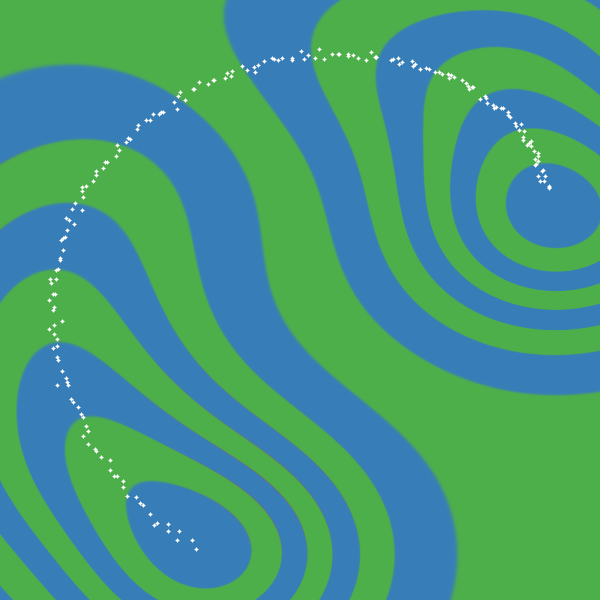
\includegraphics[width=0.45\columnwidth]{figures/hidden_good} &
\begin{tikzpicture}[pile/.style={thick, ->, >=stealth'}]
    \node[anchor=south west,inner sep=0] at (0,0) {
    	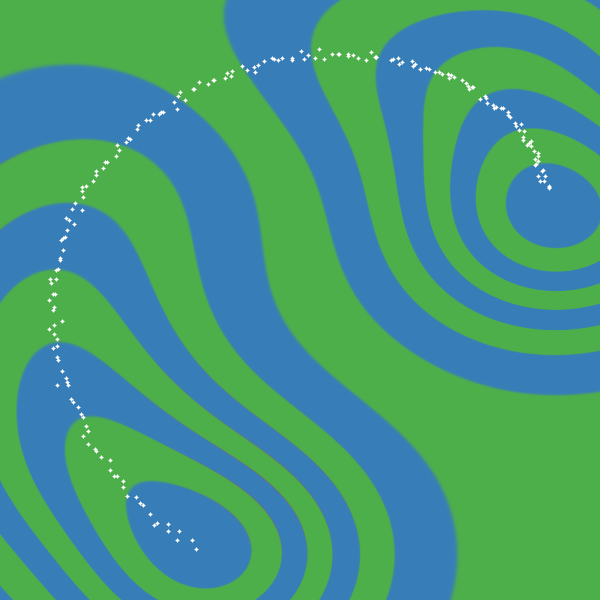
\includegraphics[clip, trim = 0cm 10cm 0cm 0.0cm, width=0.45\columnwidth]{figures/hidden_good}
    };
    \draw[pile] (2.25,1.35) coordinate (A) -- (1.6,2.1) coordinate (B) node[right, text width=5em] {};
    \fill[red]  (A)  coordinate (out) circle (2pt) {};
    \fill[white]  (B)  coordinate (out) circle (2pt) {};
    \fill[white]  (A)  coordinate (out) node[below right] {noisy point};
    \fill[white]  (B)  coordinate (out) node[right] {\quad equivalent point};
    \draw[pile] (A) -- (B) node {};
%    \draw[red,ultra thick,rounded corners] (4,5.3) rectangle (9.4,6.2);
\end{tikzpicture} &
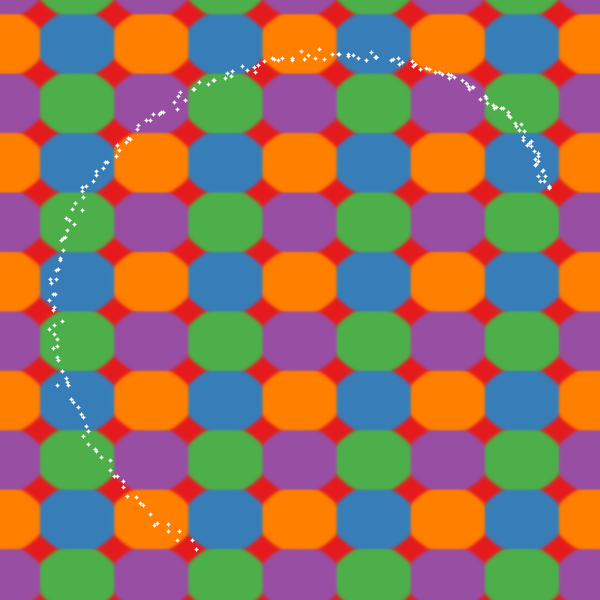
\includegraphics[clip, trim = 0cm 10cm 0cm 0.0cm, width=0.45\columnwidth]{figures/hidden_bad} \\
A compact, noise-tolerant latent representation & A na\"{i}ve latent representation \\
of a one-dimensional manifold & of a one-dimensional manifold
\end{tabular}
\caption{Comparing different latent representations of data on a 1-D manifold.  A good latent representation is invariant in directions orthogonal to the data manifold, making the representation robust to noise in those directions.  The representation must also change in directions tangent to the manifold, in order to preserve information for later layers. }% The representation on the right might be useful if the data were spread out in over plane.}
\label{fig:hidden}
\end{figure}
%
%We formalize the pathology in two ways:  One, by the distribution of the magnitude of derivatives, and two, by the relative magnitudes of singular vectors of the Jacobian.
%
We follow \cite{rifai2011contractive} in characterizing the representational properties of a function by the singular value spectrum of the Jacobian\footnote{ \cite{rifai2011contractive} examine the Jacobian at the training points, but the models we are examining are stationary, so it doesn't matter where we examine the function.}.  

\begin{figure}[h]
\centering
\begin{tabular}{ccc}
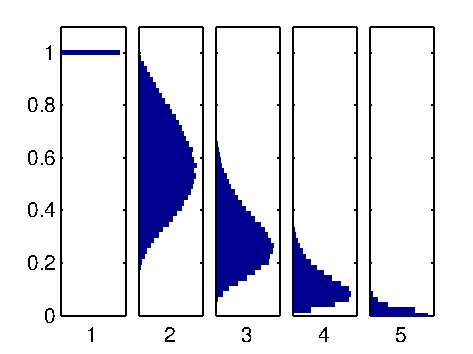
\includegraphics[width=0.315\columnwidth]{figures/spectrum/layer-2} &
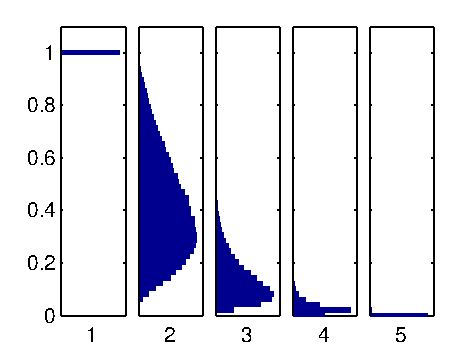
\includegraphics[width=0.315\columnwidth]{figures/spectrum/layer-4} &
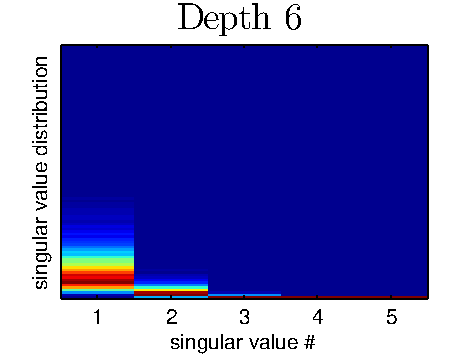
\includegraphics[width=0.315\columnwidth]{figures/spectrum/layer-6} 
%2 layers & 4 layers & 6 layers
\end{tabular}
\caption{Normalized singular value spectrum of the Jacobian of a deep GP.  As the net gets deeper, the largest singular value dominates.  This implies that there is only one effective degree of freedom in the representation being computed.}
\label{fig:deep_spectrum}
\end{figure}
%
Figure \ref{fig:deep_spectrum} shows the spectrum for 5-dimensional deep GPs of different depths.  As the net gets deeper, the largest singular value dominate, implying there is usually only one effective degree of freedom in representation being computed.  As well, the distribution on singular vlaues becomes heavy-tailed.

%
\newcommand{\gpdrawbox}[1]{
\setlength\fboxsep{0pt}
\hspace{-0.2in} 
\fbox{
\includegraphics[width=0.232\columnwidth]{figures/deep_draws/deep_gp_sample_layer_#1}
}}
\begin{figure}[h!]
\centering
\begin{tabular}{cccc}
\gpdrawbox{1} &
\gpdrawbox{2} &
\gpdrawbox{4} & 
\gpdrawbox{6} \\
%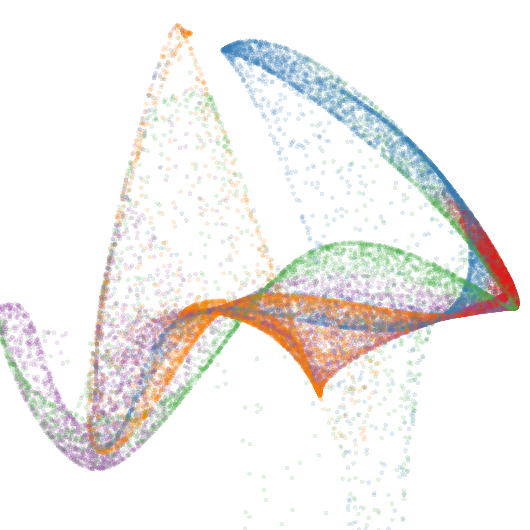
\includegraphics[width=0.3\columnwidth]{figures/deep_draws/deep_gp_sample_layer_3} \\
%$p(\vx)$ & $p(f_1(\vx))$ & $p(f_2(f_1(\vx)))$ \\ \\
%\fbox{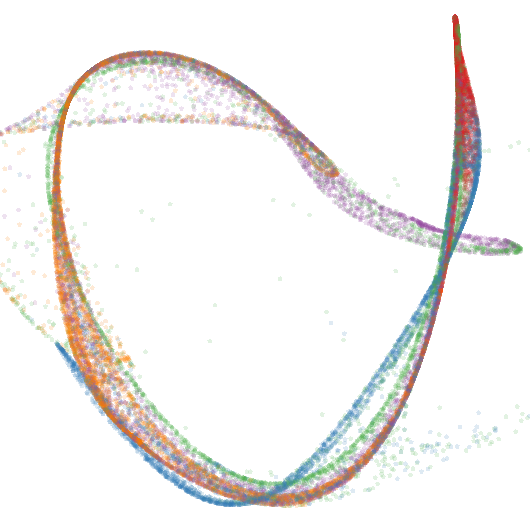
\includegraphics[width=0.24\columnwidth]{figures/deep_draws/deep_gp_sample_layer_4}} &
%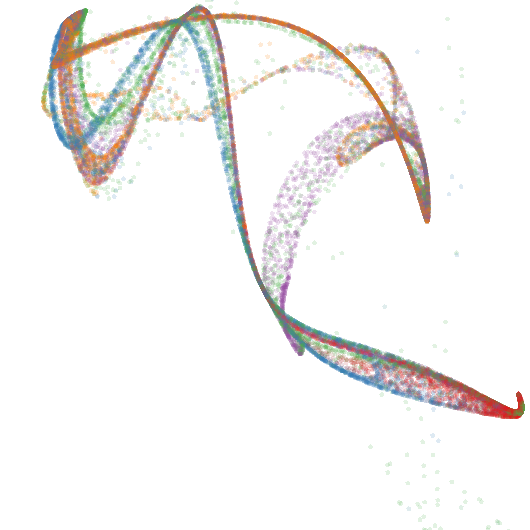
\includegraphics[width=0.3\columnwidth]{figures/deep_draws/deep_gp_sample_layer_5} &
%\fbox{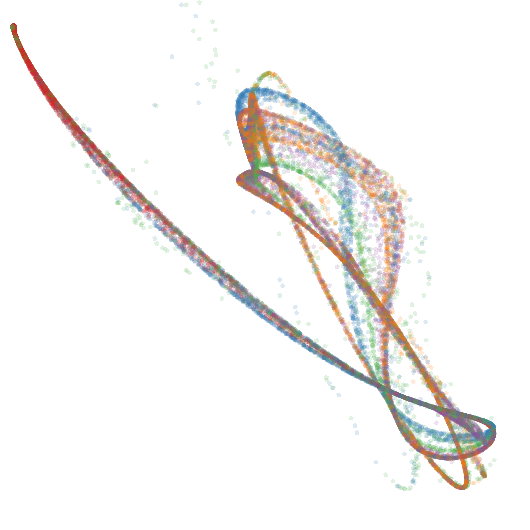
\includegraphics[width=0.24\columnwidth]{figures/deep_draws/deep_gp_sample_layer_6}} \\
%$p(f_3(f_2(f_1(\vx))))$ & $p(f_4(f_3(f_2(f_1(\vx)))))$ & $p(f_5(f_4(f_3(f_2(f_1(\vx)))))$
$p(\vx)$ & $p(f^1(\vx))$ & $p(f^{1:4}(\vx))$ &  $p(f^{1:6}(\vx))$ \\
\end{tabular}
\caption{Draws from a deep GP.  A distribution is warped by successive functions drawn from a \gp{} prior.  As the number of layers increases, the density exhibits a sort of filamentation.}
\label{fig:filamentation}
\end{figure}
%
Figure \ref{fig:filamentation} demonstrates a related pathology that arises when composing functions to produce a deep latent-variable model.  The density in observed space eventually becomes locally concentrated onto one-dimensional manifolds, or \emph{filaments}.

\newcommand{\mappic}[1]{\hspace{-0.05in}\includegraphics[width=0.23\columnwidth]{figures/map/latent_coord_map_layer_#1}} 
\newcommand{\mappiccon}[1]{\hspace{-0.05in} \includegraphics[width=0.23\columnwidth]{figures/map_connected/latent_coord_map_layer_#1}}
\begin{figure}[h!]
\centering
\begin{tabular}{cccc}
\mappic{0} & \mappic{1} & \mappic{2} & \mappic{40} \\
Identity Map: $\vy = \vx$ & 1 Layer: $\vy = f^1(\vx)$ & 2 Layers: $\vy = f^{1:2}(\vx)$ & 40 Layers %\\2 Layers: $\vy = f_1(f_2(\vx))$ \\
%\mappic{4} & \mappic{10} & \mappic{40} \\
%4 Layers & 10 Layers & 
\end{tabular}
\caption{Feature Mapping of a deep GP.  Shown here are the colors corresponding to the location $\vy = f(\vx)$ that each point is mapped to after being warped by a deep GP.  %This figure can be seen as the inverse of figure \ref{fig:filamentation}.  
Just as the densities in \ref{fig:filamentation} became locally one-dimensional, there is locally only one direction that one can move $\vx$ in to change $\vy$.  Regions where the colors change rapidly indicate that the Jacobian is large in that area.}
\label{fig:deep_map}
\end{figure}
%
To visualize this pathology in another way, figure \ref{fig:deep_map} illustrates the value that at each point in the input space is mapped to, after successive warpings.  After 40 warpings, we can see that locally, there is usually only one direction that one can move in $\vx$-space in order to change the value of the function.

To what extent are these pathologies present in nets being used today?  In simulations, we found that for deep functions with a fixed latent dimension $D$, the singular value spectrum remained relatively flat for hundreds of layers as long as $D > 100$.  Thus, these pathologies are unlikely to severely affect relatively shallow, wide networks.


\section{Fixing the pathology}
\label{sec:fix}

Follow a suggestion from \cite{neal1995bayesian}, we can fix the pathologies exhibited in figures \ref{fig:filamentation} and \ref{fig:deep_map} by simply making each layer of depend not only on the output of the previous layer, but also on the original input $\vx$.  Draws from the resulting priors are shown in figures \ref{fig:no_filamentation} and \ref{fig:deep_map_connected} and \ref{fig:deep_draw_1d_connected}.
%
\begin{figure}[h!]
\centering
\begin{tabular}{cccc}
\hspace{0.05in}
\onedsamplepiccon{1} &
\onedsamplepiccon{2} &
\onedsamplepiccon{5} &
\onedsamplepiccon{10}
%& 6 layers \\ & largest , for unconnected layers & largest, for connected layers
\end{tabular}
\caption{One-dimensional draws from a deep \gp{} prior with eeach layer connected to the input. Even after many layers, the functions remain smooth in some regions, while varying rapidly in other regions.}
\label{fig:deep_draw_1d_connected}
\end{figure}
%
%Figure \ref{fig:deep_draw_1d_connected} shows draws from a 1D deep \gp{} prior with a connected architecture.

%\begin{figure}
%\centering
%\begin{tabular}{ccc}
%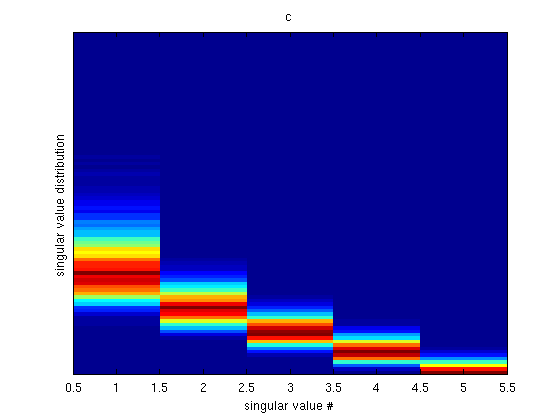
\includegraphics[width=0.3\columnwidth]{figures/spectrum/svd_specturm_depth_50_connected} &
%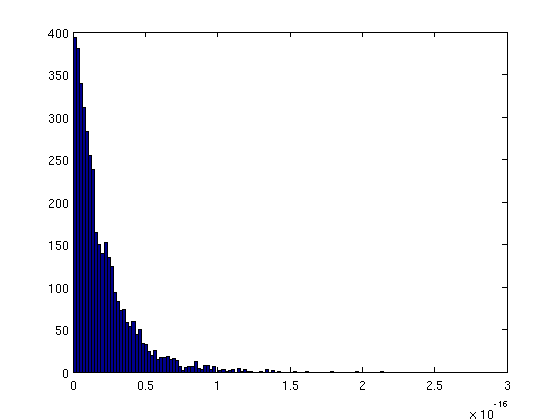
\includegraphics[width=0.3\columnwidth]{figures/spectrum/svd_ratio_depth_50} &
%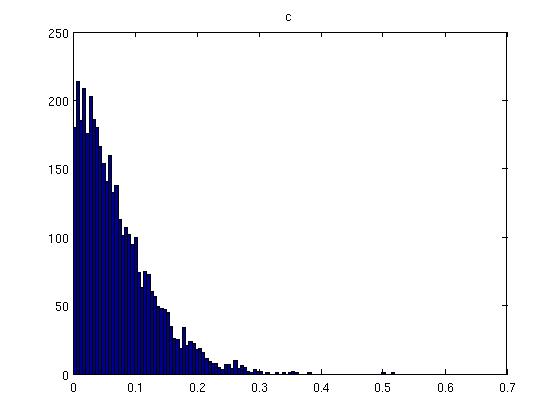
\includegraphics[width=0.3\columnwidth]{figures/spectrum/svd_ratio_depth_50_connected} \\
%50 connected layers & smallest singular value divided by & 6 layers \\
% & largest , for unconnected layers & largest, for connected layers
%\end{tabular}
%\caption{Reparing the singular value distribution.  When each layer is connected to the original inputs, and the variance of derivatives is smaller than a threshold, then the ratio of the largest singular value to the smallest remains small.}
%\label{fig:deep_spectrum_fixed}
%\end{figure}



%
%
\begin{figure}[h!]
\centering
\begin{tabular}{cccc}
\hspace{-0.07in} \mappic{0} & \mappiccon{2} & \mappiccon{10} & \mappiccon{40} \\
Identity Map: $\vy = \vx$ & 2 connected Layers & 10 Connected Layers & 40 Connected Layers %\\2 Layers: $\vy = f_1(f_2(\vx))$ \\
%\mappic{4} & \mappic{10} & \mappic{40} \\
%4 Layers & 10 Layers & 
\end{tabular}
\caption{Feature Mapping of a deep GP with each layer connected to the input $\vx$.  Just as the densities in \ref{fig:no_filamentation} became remain locally two-dimensional even after many transformations, in this mapping there are locally usually two directions that one can move in $\vx$ to change $\vy$.}
\label{fig:deep_map_connected}
\end{figure}





\paragraph{Jacobians of connected deep networks}

\newcommand{\gpdrawboxcon}[1]{
\setlength\fboxsep{0pt}
\hspace{-0.2in} 
\fbox{
\includegraphics[width=0.232\columnwidth]{figures/deep_draws_connected/deep_sample_connected_layer#1}
}}
\begin{figure}[h!]
\centering
\begin{tabular}{cccc}
%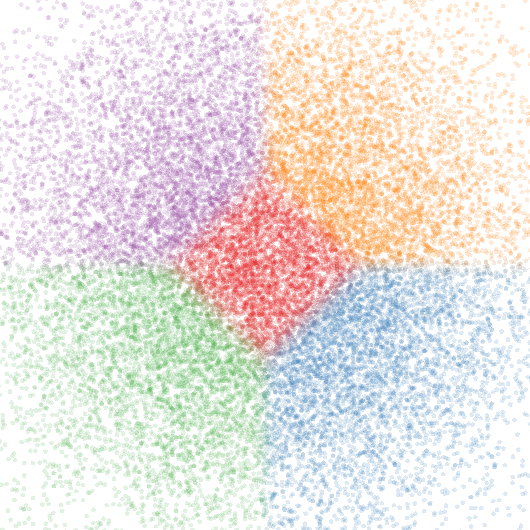
\includegraphics[width=0.3\columnwidth]{figures/deep_draws/deep_gp_sample_layer_1} &
%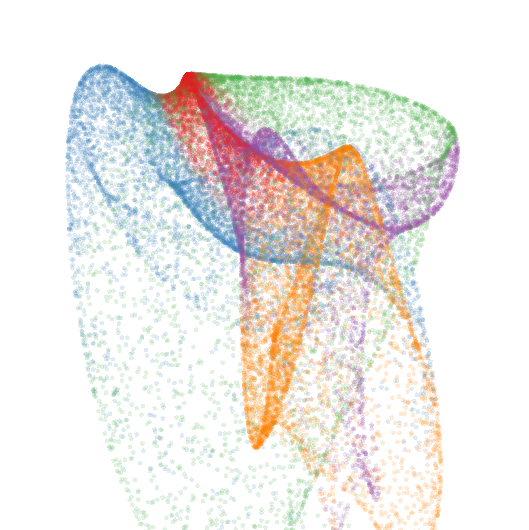
\includegraphics[width=0.3\columnwidth]{figures/deep_draws_connected/deep_sample_connected_layer2} &
%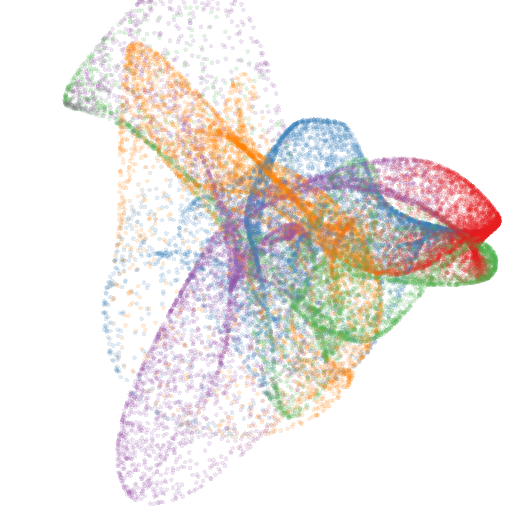
\includegraphics[width=0.3\columnwidth]{figures/deep_draws_connected/deep_sample_connected_layer3} \\
%$p(\vx)$ & $p(f_1(\vx))$ & $p(f_2(f_1(\vx), \vx))$ \\ \\
%\gpdrawboxcon{2} &
\gpdrawboxcon{4} &
\gpdrawboxcon{5} &
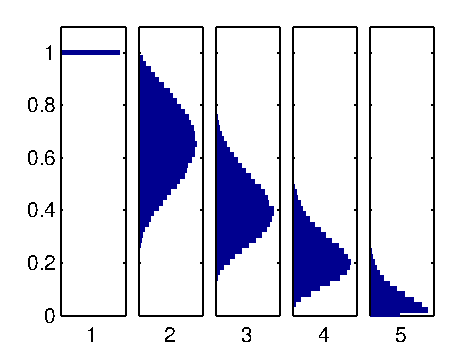
\includegraphics[width=0.315\columnwidth]{figures/spectrum/con-layer-50} \\
%\gpdrawboxcon{6} \\
 4 Layers & 5 Layers & Singular Value Spectrum
%$p(f_3(f_2(f_1(\vx),\vx),\vx))$ & $p(f_4(f_3(f_2(f_1(\vx), \vx),\vx),\vx))$ & $p(f_5(f_4(f_3(f_2(f_1(\vx),\vx),\vx),\vx),\vx))$
\end{tabular}
\caption{Left: Densities defined by a draw from a deep GP, with each layer connected to the input $\vx$.  As depth increases, the density becomes more complex without concentrating along filaments. Right:  The singular value spectrum of a 6-dimensional deep \gp{} prior 50 layers deep.  The singular values remain roughly the same scale.}
\label{fig:no_filamentation}
\end{figure}

We can similarily examine the Jacobians of the new connected architecture.  The Jacobian of a composite function which has had the original inputs appended 
$f_\textnormal{aug}(\vx) = [ f(\vx), \vx ]$,
is 
%$ \left[J_f \quad I_D \right] $
$ \left[ \! \begin{array}{c} J_f \\ I_D  \end{array} \! \right] $
 and the Jacobian of all one-layer transformations of these augmented functions are $D \times 2D$ matrices.
The Jacobian of the composed, connected deep function is defined by the recurrence:
%
\newcommand{\sbi}[2]{\left[ \! \begin{array}{c} #1 \\ #2 \end{array} \! \right]} 
%\newcommand{\sbi}[2]{\left[ #1 \quad \!\! #2 \right]} 
%\begin{align}
$J^{1:L}(\vx) = J^L \sbi{ J^{1:L-1}}{I_D}$
%\end{align}
%
%So the entire Jacobian has the form:
%
%\begin{align}
%J^{1:L}(x) = J^L \sbi{ J^{L-1} \sbi{ \dots J^{4} \sbi{ J^{3} \sbi{ J^2 J^1 }{ I_D }}{ I_D } \dots }{ I_D \\ \vdots }}{ I_D}
%\end{align}
%
Figure \ref{fig:no_filamentation} shows that with this architecture, even 50-layer deep \gp{}s have well-behaved singular value spectra.






\section{Arbitarily Deep Kernels}
\label{sec:deep_kernels}

\cite{cho2012kernel} investigated kernels constructed by applying multiple layers of feature mappings.  That is to say, if a kernel has the form $k_1(\vx, \vx') = \Phi(\vx) \tra \Phi(\vx)$, then we can consider constructing a kernel based on the repeated feature mapping: $k_2(\vx, \vx') = k_2(\Phi(\vx), \Phi(\vx')) = \Phi(\Phi(\vx)) \tra \Phi(\Phi(\vx))$.
%
%We can consider applying the feature transform $\Phi(\cdot)$ to the features themselves:  $\Phi_2 = \Phi(\Phi(\vx))$.  

For the squared-exp kernel, this composition operation has a closed form:% for any set of starting features $\Phi_n(\vx)$:
%
%In this section, we take the infinite limits of these compositions, and propose a new variant.
%
%One can derive a Gaussian process as a neural network: $f(x) = {\mathbf \alpha}^T \Phi(x) = \sum_{i=i}^K \alpha_i \phi_i(x)$.  
%
%
%we derive a kernel which corresponds to arbitrarily many compositions of the feature vectors corresponding to the squared-exp kernel:
%
\begin{align}
%k_1(\vx, \vx') & = \exp \left( -\frac{1}{2} ||\vx - \vx'||_2^2 \right) \\
k_{n+1}(\vx, \vx') & = \exp \left( -\frac{1}{2} || \Phi_n(\vx) - \Phi_n(\vx')||_2^2 \right) \\
k_{n+1}(\vx, \vx') & = \exp \left( -\frac{1}{2} \sum_i \left[ \phi_n^{(i)}(\vx) - \phi_n^{(i)}(\vx') \right]^2 \right) \\
%k_2(\vx, \vx') & = \exp\left ( -\frac{1}{2} \sum_i \left[ \phi_i(\vx)^2 - 2 \phi_i(\vx) \phi_i(\vx') + \phi_i(\vx')^2 \right] \right) \\
%k_2(\vx, \vx') & = \exp \left( -\frac{1}{2} \left[ \sum_i \phi_i(\vx)^2 - 2 \sum_i \phi_i(\vx) \phi_i(\vx') + \sum_i \phi_i(\vx')^2 \right] \right) \\
k_{n+1}(\vx, \vx') & = \exp \left( -\frac{1}{2} \left[ k_n(\vx, \vx) - 2 k_n(\vx, \vx') + k_n(\vx', \vx') \right] \right)\\
k_{n+1}(\vx, \vx') & = \exp \left( k_n(\vx, \vx') - 1 \right) \qquad \textnormal{(if $k_n(\vx, \vx) = 1$)}
\end{align}
%
%\begin{figure}
%\centering
%\begin{tabular}{ccc}
%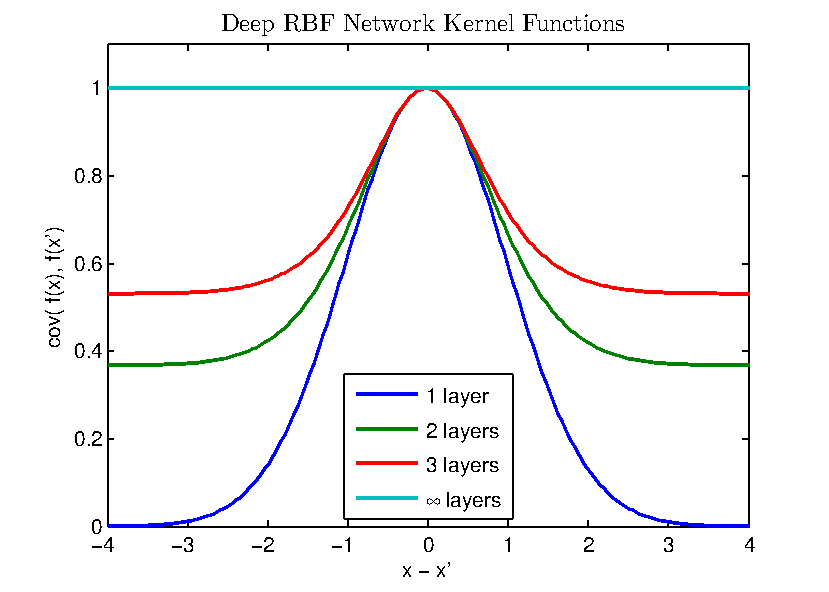
\includegraphics[width=0.5\columnwidth, clip, trim = 0cm 0cm 0cm 0.61cm]{figures/deep_kernel} &
%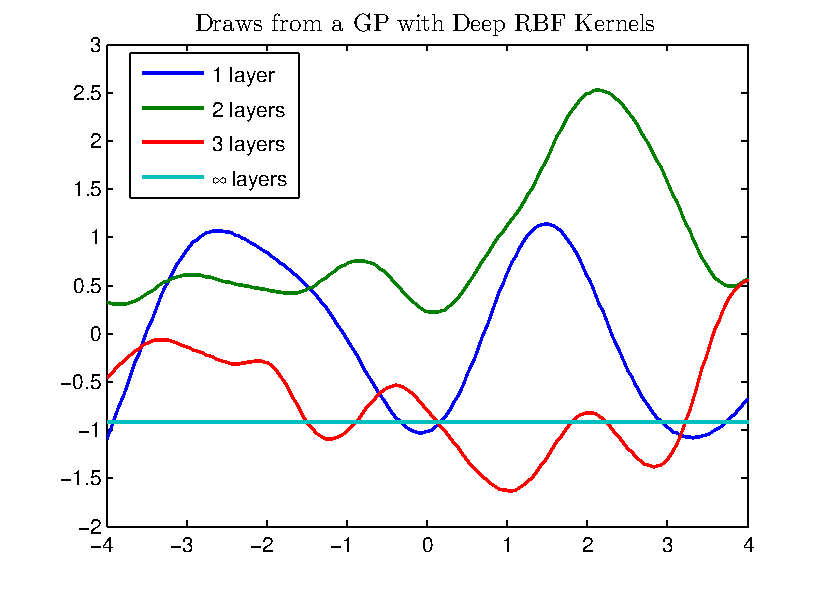
\includegraphics[width=0.5\columnwidth, clip, trim = 0cm 0cm 0cm 0.61cm]{figures/deep_kernel_draws} \\
%Kernel derived from iterated feature transforms & Draws from the corresponding kernel
%\end{tabular}
%\caption{A degenerate kernel produced by repeatedly applying a feature transform.}
%\label{fig:deep_kernel}
%\end{figure}
%
%Thus, if $k_1(x,y) = e^{-||x - y||2}$, then the two-layer kernel is simply $k_2(x,y) = e^{k_1(x, y) - 1}$.  This formula is true for every layer: $k_{n+1}(x,y) = e^{k_n(x, y) - 1}$.
%
%Note that nothing in this derivation depends on details of $k_n$, except that $k_n( \vx, \vx) = 1$.
Note that this result holds for any base kernel $k_n$, as long as $k_n( \vx, \vx) = 1$.
%  Because this is true for $k_2$ as well, this recursion holds in general, and we have that $k_{n+1}(x,y) = e^{k_n(x, y) - 1}$.  

\paragraph{Infinitely deep kernels}
What happens when we apply this compsition many times, starting with the squared-exp kernel?  In the infinite limit, this recursion converges to $k(x,y) = 1$ for all pairs of inputs.  Figure \ref{fig:deep_kernel_connected} shows this kernel at different depths, including the degenerate limit.  

One interpretation of why repeated feature transforms lead to this degenerate prior is that each layer can only lose information about the previous set of features.  In the limit, the transformed features contain no information about the original input $\vx$.  Since the function doesn't depend on its input, it must be the same everywhere.

\paragraph{A non-degenerate construction}

Again, following a suggestion from \cite{neal1995bayesian}, we connect the inputs $\vx$ to each layer.  To do so, we simply augment the feature vector $\Phi_n(\vx)$ with the $\vx$ at each layer:
%
\begin{align}
%k_1(\vx, \vx') & = \exp \left( -\frac{1}{2} ||\vx - \vx'||_2^2 \right) \\
k_{n+1}(\vx, \vx') & = \exp \left( -\frac{1}{2} \left|\left| \left[ \! \begin{array}{c} \Phi_n(\vx) \\ \vx \end{array} \! \right]  - \left[ \! \begin{array}{c} \Phi_n(\vx') \\ \vx' \end{array} \! \right] \right| \right|_2^2 \right) \\
k_{n+1}(\vx, \vx') & = \exp \left( -\frac{1}{2} \sum_i \left[ \phi_i(\vx) - \phi_i(\vx') \right]^2 -\frac{1}{2} || \vx - \vx' ||_2^2 \right) \\
%k_{n+1}(\vx, \vx') & = \exp\left ( -\frac{1}{2} \sum_i \left[ \phi_i(\vx)^2 - 2 \phi_i(\vx) \phi_i(\vx') + \phi_i(\vx')^2 \right]  -\frac{1}{2} || \vx - \vx' ||_2^2 \right) \\
%k_2(\vx, \vx') & = \exp \left( -\frac{1}{2} \left[ \sum_i \phi_i(\vx)^2 - 2 \sum_i \phi_i(\vx) \phi_i(\vx') + \sum_i \phi_i(\vx')^2 \right] \right) \\
%k_2(\vx, \vx') & = \exp \left( -\frac{1}{2} \left[ k_1(\vx, \vx) - 2 k_1(\vx, \vx') + k_1(\vx', \vx') \right] \right) \\
k_{n+1}(\vx, \vx') & = \exp \left( k_n(\vx, \vx') - 1 -\frac{1}{2} || \vx - \vx' ||_2^2 \right)
\end{align}
%
%
This kernel satisfies the recurrence $k - \log(k) = 1 + \frac{1}{2} || \vx - \vx' ||_2^2$, a non-degenerate limit.  The solution to this recurrence has no closed form, but it is continuous and differentiable everywhere except at $\vx = \vx'$.
%
Samples from a \gp{} with this prior are not differentiable, and locally resemble brownian motion, having a sort of fractal behavior.

%\item This kernel has smaller correlation than the squared-exp everywhere except at $\vx = \vx'$.  
%\item Samples from this kernel are fractal.
%\item The tails have the same form as the squared-exp.
%\end{itemize}

\begin{figure}[h]
\centering
\begin{tabular}{ccc}
\hspace{-0.5cm}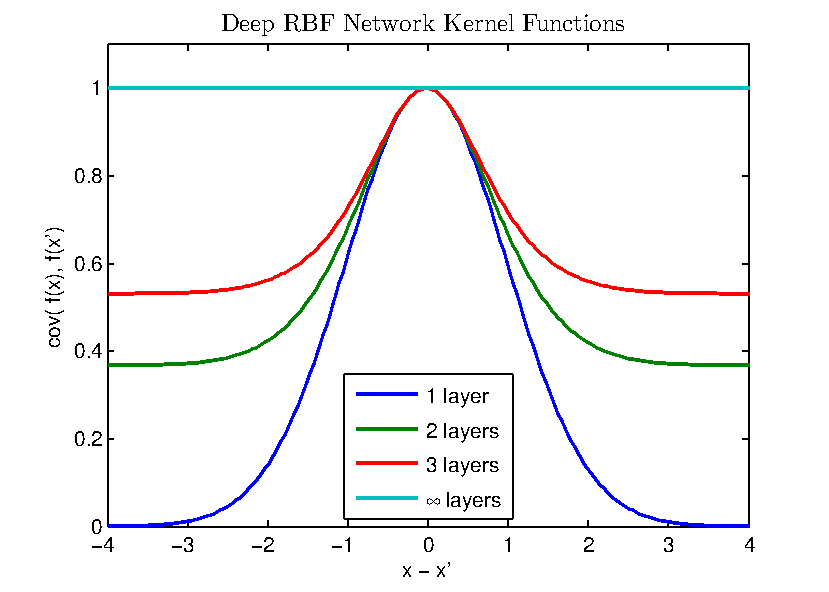
\includegraphics[width=0.35\columnwidth, clip, trim = 0cm 0cm 0cm 0.61cm]{figures/deep_kernel} &
\hspace{-0.5cm}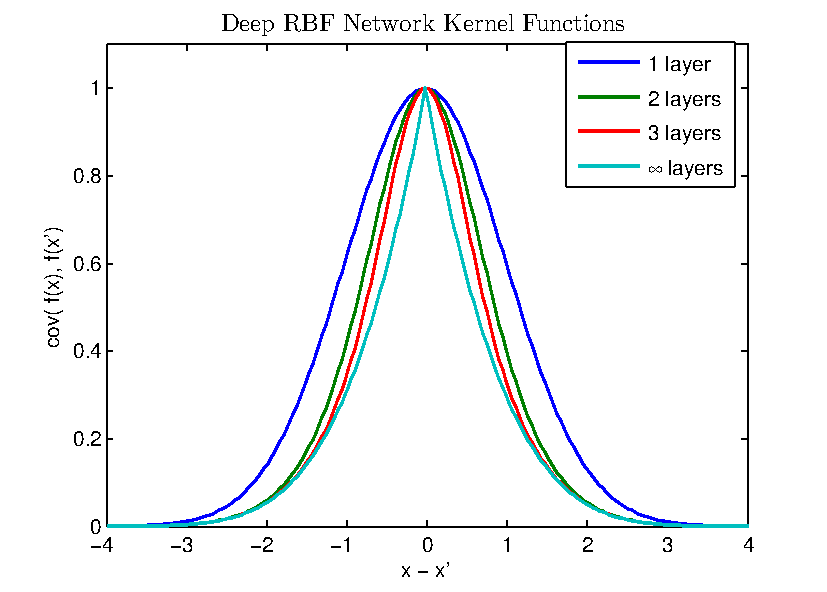
\includegraphics[width=0.35\columnwidth, clip, trim = 0cm 0cm 0cm 0.61cm]{figures/deep_kernel_connected} &
\hspace{-0.5cm}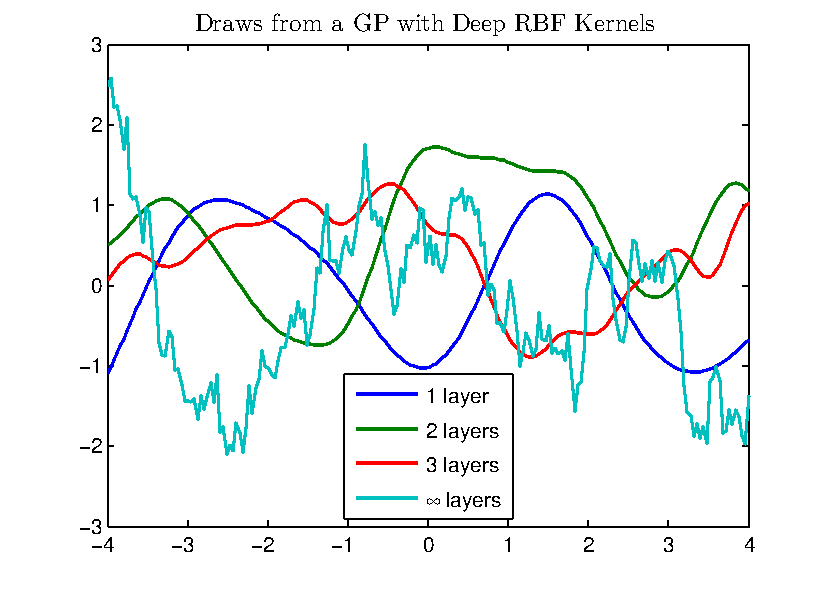
\includegraphics[width=0.35\columnwidth, clip, trim = 0cm 0cm 0cm 0.61cm]{figures/deep_kernel_connected_draws} \\
Iterated transform kernel & Connected transform kernel & Connected \gp{} draws
\end{tabular}
\caption{Left: A kernel corresponding to composing features.  In the limit, it becomes degenerate.  Center: A non-degenerate version of the infinitely deep feature transform kernel.  By connecting the inputs $\vx$ to each layer, the function can still depend on its input even after arbitrarily many layers of computation.  Right: Draws from this kernel.}
\label{fig:deep_kernel_connected}
\end{figure}


%\subsection{A fully-connected kernel}
%However, connecting every layer to every subsequent layer leades to a pathology:
%\begin{align}
%k_1(\vx, \vx') & = \exp \left( -\frac{1}{2} ||\vx - \vx'||_2^2 \right) \\
%k_{n+1}(\vx, \vx') & = \exp \left( -\frac{1}{2} \left|\left| \left[ \! \begin{array}{c} \Phi_n(\vx) \\ \Phi_{n-1}(\vx') \end{array} \! \right]  - \left[ \! \begin{array}{c} \Phi_n(\vx') \\ \Phi_{n-1}(\vx') \end{array} \! \right] \right| \right|_2^2 \right) \\
%k_{n+1}(\vx, \vx') & = \exp \left( -\frac{1}{2} \sum_i \left[ \phi^{(i)}_n(\vx) - \phi^{(i)}_n(\vx') \right]^2 -\frac{1}{2} \sum_i \left[ \phi^{(i)}_{n-1}(\vx) - \phi^{(i)}_{n-1}(\vx') \right]^2 \right)\\
%k_{n+1}(\vx, \vx') & = \exp\left ( -\frac{1}{2} \sum_i \left[ \phi_i(\vx)^2 - 2 \phi_i(\vx) \phi_i(\vx') + \phi_i(\vx')^2 \right]  -\frac{1}{2} || \vx - \vx' ||_2^2 \right) \\
%k_2(\vx, \vx') & = \exp \left( -\frac{1}{2} \left[ \sum_i \phi_i(\vx)^2 - 2 \sum_i \phi_i(\vx) \phi_i(\vx') + \sum_i \phi_i(\vx')^2 \right] \right) \\
%k_2(\vx, \vx') & = \exp \left( -\frac{1}{2} \left[ k_1(\vx, \vx) - 2 k_1(\vx, \vx') + k_1(\vx', \vx') \right] \right) \\
%k_{n+1}(\vx, \vx') & = \exp \left( k_n(\vx, \vx') - 1 \right) \exp \left( k_{n-1}(\vx, \vx') - 1 \right)
%k_{n+1}(\vx, \vx') & = \prod_{i=1}^n \prod_{j=1}^i \exp \left( k_i(\vx, \vx') - 1 \right)
%\end{align}
%Which has the solution $k_\infty = \delta( \vx = \vx' )$, a white noise kernel.


%\subsection{Connecting every layer to the end}
%There is a fourth possibilty (suggested by Carl), of connecting every layer to the output:
%\begin{align}
%k_n(\vx, \vx') & = \exp \left( -\frac{1}{2} || \Phi_n(\vx) - \Phi_n(\vx')||_2^2 \right) \\
%k_{n+1}(\vx, \vx') & = \exp \left( k_n(\vx, \vx') - 1 \right) \\
%k_{L}(\vx, \vx') & = \prod_{i=1}^L \exp \left( k_i(\vx, \vx') - 1 \right)
%\end{align}
%Which also has the solution $k_\infty = \delta( \vx = \vx' )$, a white noise kernel.


\subsection{Can deep kernels be useful models?}

\cite{NIPS2005_424} showed that kernel machines, such as \gp{}s, have limited generalization ability when they use a local kernel such as the squared-exp.  However, many interesting non-local kernels can be constructed which allow non-trivial extrapolation, for example, periodic kernels. A periodic kernel can be viewed as a 2-layer-deep kernel, in which the first layer maps the input $x \rightarrow [\sin(x), \cos(x)]$, and the second layer maps through a set of radial-basis functions.  

Kernels can capture many other types of generalization
%cite{DuvLloGroetal13, wilsonadams2013}
, such as translation and rotation invariance in images \cite{kondor2008group}.  \cite{SalHin08} even uses a deep neural network to learn feature transforms for kernels, which learn invariances in an unsupervised manner.  
%
In contrast, the relatively uninteresting properties of the kernels derived in this section suggest that an arbitrary deep computation not necessarily powerful unless combined with learning.  For any specific problem, an arbitrary set of computations are unlikely to lead to useful generalization. % - many layers of computation are 

%\paragraph{More general feature compositions}
%The results in this section show how to map any kernel's features through an RBF feature mapping in closed form, and also how to append any other set of features to such a kernel.  We can combine these results to define kernels corresponding to arbitrary fixed computation graphs.  Learning such computation graphs may be a useful model-construction technique.


\section{Related Work}

Variational inference in deep Gausian processes was developed by \cite{damianou2012deep}, who also analyzed the effect of ARD in these models.
%
%\subsection{A Survey of deep architectures}
%
Besides deep \gp{}s, other variants of deep models have been proposed, such as Bayesian Deep Networks \cite{adams2010learning}.% and Sum-product networks \cite{poon2011sum}  
%developed a prior on finite but unboundedly deep neural networks, each layer having a finite but unbounded number of hidden units.  
These models have no connections except between adjacent layers, and may also be expected to have similar pathologies to deep \gp{} as the number of layers increases.
%
Deep Density Networks \cite{rippel2013high} were constructed with invertibility in mind, with penalty terms encouraging the preservation of information about lower layers.


%\paragraph{Feature Composition Kernels} \cite{cho2012kernel} developed kernels of the type discussed in section \ref{sec:deep_kernels}, and investigated them experimentally.

%\cite{pascanu2012understanding} analyze the exploding-gradients problem in recurrent neural networks.

%\paragraph{Dynamical Systems}
%These architectures are all constructed in a stacked manner, with connections only between adjacent layers.

%\subsection{Related Analyses}

\cite{montavon2010layer} perform a layer-wise analysis of deep networks, and note that the performance of MLPs degrades as the number of layers with random weights increases.
%\url{http://books.nips.cc/papers/files/nips23/NIPS2010_0206.pdf}

%\section{Discussion}

%\subsection{Deep GPs for supervised learning}
%So, far, deep Guassian processes have been used mainly in latent variable models \cite{damianou2012deep}.  However, we can begin to think about their properties for supervised tasks.

%\paragraph{Recursive learning method}
%Just as layer-wise unsupervised pre-training encourages the projection of the data into a representation with independent features in the higher layers, so does the procedure outlined here.  This is because the isotropic kernel does not penalize independence between different dimensions, only the number of dimensions.


\section{Conclusions}

In this paper, we have shown the following propositions:

\begin{itemize}
\item Deep \gp{}s can be viewed as MLPs with a finite number of nonparametric hidden units.
\item Deep \gp{}s can be chracterized using random matrix theory.
\item Representations based on repeated composition of independently-initialized functions exhibit a pathology where the representation becomes invariant to all but one direction of variation.
%\item If you initialize independently, the density becomes fractal.
\item Connecting the input to each layer of a deep representation produces allows us to construct priors on deep functions without this pathology.
% Points close in $x$-space can be very far in $y$-space, and vice versa.
\end{itemize}

This analysis is simply a first step in constructing useful priors over deep functions.  Future work could also include relating automatic relevance determination to sparse regularization methods, or variational inference in deep \gp{}s to dropout-related regularization.


\subsubsection*{Acknowledgments}
We thank Carl Rasmussen, Andrew McHutchon, Neil Lawrence, Andreas Diamanadou, James Lloyd, Creighton Heaukulani, Dan Roy and Mark van der Wilk for helpful discussions.


\bibliographystyle{unsrt}
\bibliography{verydeep}


\end{document}




















\paragraph{Attempted definition of a filament}  A continuous, twice-differentiable region of a pdf is called a \emph{filament} to the degree that, weighted by density, only one eigenvalue of the Hessian of the pdf are is small relative to the average eigenvalue.


\paragraph{Approach}
We are going to analyze these networks by looking at the neighbourhood surrounding random points.

\subsection{Different settings}

In our analysis, we assume that functions are normalized.



\begin{itemize}
\item The kernel is an RBF, meaning that all functions are infinitely differentiable.  This also corresponds to the infinite limit taken by Radford Neal [cite]
\item The dimension of the latent space is always the same.
\end{itemize}

We consider several different variations of deep GPs:

\begin{itemize}
\item mean function $m_d(x_d) = 0$
\item mean function $m_d(x_d) = x_d$
\end{itemize}

\paragraph{Noise versus no noise}
Do the deep functions we're interested in modeling have noise added at each step?  Consider the example of handwritten digits.  One putative model would be that $x$ is the number that the human is trying to write, then a series of functions of his nervous system and arm (with feedback loops) cascade to produce the observed digit.  This whole process can be expected to have small amounts of noise at each step, but presumably \emph{can only work if the amount of noise is small}.

A function whose result gets a lot of noise added at each intermediate step is probably not useful unless there is an error-correcting step applied downstream.  Perhaps our results hold because random functions do not do error-correction.  Perhaps this is another intuition for why 'dropout' works - functions are explicitly trained to be robust to noise.  Denoising autoencoders are also trained in this way.

\begin{itemize}
\item Density models
\item Function models
\end{itemize}




\begin{align}
\textrm{Filament}(p(\vx)) = 1 - \int \frac{ \bar \lambda}{ \lambda_\textrm{min}} p(\vx) d\vx
\end{align}

where $\lambda_\textrm{min}$ is the smallest eigenvalue of the Hessian of $p(\vx)$.

There is some sort of connection between average eigenvalue and signal power:
[\url{http://www1.i2r.a-star.edu.sg/~yhzeng/ZENG-TCOM-09-0402.pdf}]

This definition doesn't depend on scale, although it does depend on parameterization in general.

\paragraph{Example: A uniform distribution of any dimension}
A uniform distribution has $\textrm{Filament}(p(\vx)) = 0$.

\paragraph{Example: Any distribution defined over 1 dimension}
In one dimension, there is only one eigenvalue, so $ \bar \lambda = \lambda_\textrm{min}$, and thus $\frac{ \bar \lambda}{ \lambda_\textrm{min}} = 1$ everywhere.  So every 1D distribution has $\textrm{Filament}(p(\vx)) = 0$.

\paragraph{Example: A 1D sigmoid in two dimensions}
A 1d sigmoidal-shaped distribution in two dimensions will have $\textrm{Filament}(p(\vx)) > 0$, because at the top of the curve, $\frac{ \bar \lambda}{ \lambda_\textrm{min}} > 1$, and this can't be cancelled out, because everywhere else, $\frac{ \bar \lambda}{ \lambda_\textrm{min}} \geq 1$.

\subsection{Why does filamentation occur?}
Intuition: The space will be squished in some directions, and stretched in others.  However, any direction's Jacobian will be a product of lots of directional Jacobians.  This distribution will become heavy-tailed, meaning that it will be dominated by a few small values.  We can characterize the ratio of the maximum direction of curvature to the average.




\paragraph{The Hessian of a deep density model}

Since we know the density of a point drawn from a deep GP, we can also look at the local curvature through the Hessian.  Given an $\vx, \vy$ pair $\vy = f(\vx)$, 
%
\begin{align}
p(\vy) 
= \frac{p_x( f\inv(\vy ))}{\left| J( f\inv(\vy)) \right|} 
= \frac{p_x( \vx )}{\left| J( \vx) \right|}
= p_x( \vx ) \left| J( \vx)\inv \right|
\end{align}
%
So we can say that the determinant of the inverse transform $\left| J( \vx)\inv \right|$ defines the local distortion of density.

We want to know how many directions we can move in.

We could characterize this by the probability, if we moved in a random direction, of not moving into a region of low probability.  If we're at a local maximum, we can ask how many eigenvalues of the Hessian are small.


The Hessian of the determinant of the Jacobian is:
\begin{align}
H_y \left( \left| J_{\vy \rightarrow \vx} (\vy) \right| \right)
 & = \begin{bmatrix}
\dfrac{\partial^2 \detJyy}{\partial y_1^2} & \dfrac{\partial^2 \detJyy}{\partial y_1\,\partial y_2} & \cdots & \dfrac{\partial^2 \Jyy}{\partial y_1\,\partial y_n} \\[2.2ex]
\dfrac{\partial^2 \detJyy}{\partial y_2\,\partial y_1} & \dfrac{\partial^2 \detJyy}{\partial y_2^2} & \cdots & \dfrac{\partial^2 \detJyy}{\partial y_2\,\partial y_n} \\[2.2ex]
\vdots & \vdots & \ddots & \vdots \\[2.2ex]
\dfrac{\partial^2 \detJyy}{\partial y_n\,\partial y_1} & \dfrac{\partial^2 \detJyy}{\partial y_n\,\partial y_2} & \cdots & \dfrac{\partial^2 \detJyy}{\partial y_n^2}
\end{bmatrix} \\
 & = H_y \left( \left| \Jyy \right| \right) \\
 & = H_y \left( \prod_i \lambda^{\Jy}_i ( \vy) \right) \qquad \textrm{where $\lambda$ are eigenvalues of $\Jyy$}
 \\
 & = H_y \left( \prod_i \frac{1}{\lambda^{\Jx}_i ( \vx )} \right)
\end{align}
%
where $H_y$ means that the second derivatives in the Hessian are taken w.r.t. $\vy$, and $\lambda^{J\inv}_i ( \vx)$ are the eigenvalues of the Jacobian (the total derivative of $f\inv(\vy)$ w.r.t. $\vx$).

\paragraph{Derivative of determinant}
\begin{align}
\frac{\partial \det(A)}{\partial A_{ij}}= \operatorname{adj}(A)_{ji}= \det(A)(A^{-1}_{ji}) \\
\frac{\mathrm{d} \det(A)}{\mathrm{d} \alpha} =  \det(A) \operatorname{tr}\left(A^{-1} \frac{\mathrm{d} A}{\mathrm{d} \alpha}\right)
\end{align}
%
In our case, we have:
%
\begin{align}
\frac{\partial \det(\Jyy)}{\partial \vy_i} & = \det(\Jy) \trace \left(\Jx \frac{\partial \Jyy}{\partial \vy_i}\right) \\
& = \det(\Jy) \trace \left( - \Jx \Jy \frac{\partial \Jx(\vy)}{\partial \vy_i} \Jy \right) \\
& = \det(\Jy) \trace \left( - \frac{\partial \Jx(\vy)}{\partial \vy_i} \Jy \right) \\
& = \det(\Jy) \trace \left( - \frac{\partial \Jx(\vx)}{\partial \vx} \frac{\partial \vx}{\partial \vy_i} \Jy \right) \\
& = \det(\Jy) \trace \left( - \frac{\partial \Jx(\vx)}{\partial \vx} \Jy^{:,i} \Jy \right) \\
& = \det(\Jy) \trace \left( - \Jy \frac{\partial \Jx(\vx)}{\partial \vx} \Jy^{:,i} \right) \label{eqn:ddet_tractable} \\
& = \det(\Jy) \trace \left( \frac{\partial \Jy(\vy)}{\partial \vx} \right)
\label{eqn:ddet_simple}
\end{align}
%
We don't have an analytic form for \eqref{eqn:ddet_simple}, but we can compute \eqref{eqn:ddet_tractable} if we can compute the term $\frac{\partial \Jx(\vx)}{\partial \vx}$, which is just the second derivative of $\fdeep(\vx)$.

\paragraph{Derivative of SVD}
a

\url{http://www.ics.forth.gr/_publications/2000_eccv_SVD_jacobian.pdf} says that:
%
\begin{align}
\frac{\partial \det(A)}{\partial A_{ij}}= \operatorname{adj}(A)_{ji}= \det(A)(A^{-1}_{ji})
\end{align}



\paragraph{Hessian of determinant}
\begin{align}
\frac{\partial^2 \det(A)}{\partial A_{ij}\partial A_{mn}}
& = \det(A)(A^{-1}_{ji}A^{-1}_{nm} - A^{-1}_{ni}A^{-1}_{jm})
\end{align}

We can also say that

\url{http://math.stackexchange.com/questions/50386/the-hessian-of-the-determinant}

\begin{align}
\frac{\partial^2 \det(A(\vy))}{\partial y_i \partial y_j}
& = \frac{\partial^2 \det(A(\vy))}{\partial A_{ij}\partial A_{mn}} \left( \frac{\partial A_{ij}}{\partial y_i} + \frac{\partial A_{ij}}{\partial y_j} \right) \left( \frac{\partial A_{mn}}{\partial y_i} + \frac{\partial A_{mn}}{\partial y_j} \right)
%& = \det(A)(A^{-1}_{ji}A^{-1}_{nm} - A^{-1}_{ni}A^{-1}_{jm})
\end{align}

or we can try:

\begin{align}
\frac{\partial^2 \det(A(\vy))}{\partial y_i \partial y_j}
& = \frac{\partial }{\partial \vy_j} \det(\Jy) \trace \left( \frac{\partial \Jy(\vy)}{\partial \vx} \right) \\
& = \det(\Jy) \frac{\partial }{\partial \vy_j} \trace \left( \frac{\partial \Jy(\vy)}{\partial \vx} \right) 
  + \trace \left( \frac{\partial \Jy(\vy)}{\partial \vx} \right) \frac{\partial }{\partial \vy_j} \det(\Jy) \\
\end{align}

or:

\begin{align}
\frac{\partial^2 \det(A(\vy))}{\partial y_i \partial y_j}
= \det(A) & \Big[ 
          \trace \left( A\inv \frac{\partial^2 A(\vy)}{\partial \vy_i \partial \vy_j } \right) \nonumber \\
          & + \trace \left( A\inv \frac{\partial A(\vy)}{\partial \vy_i} \right) 
            \trace \left( A\inv \frac{\partial A(\vy)}{\partial \vy_j} \right) \nonumber \\
           & + \trace \left( A\inv \frac{\partial A(\vy)}{\partial \vy_i} 
                          A\inv \frac{\partial A(\vy)}{\partial \vy_j} \right)
         \Big] \\
\frac{\partial^2 \det(\Jy(\vy))}{\partial y_i \partial y_j}
= \det(\Jy) & \Big[
          \trace \left( \Jy\inv \frac{\partial^2 \Jy(\vy)}{\partial \vy_i \partial \vy_j } \right) \nonumber \\
          & + \trace \left( \Jy\inv \frac{\partial \Jy(\vy)}{\partial \vy_i} \right) 
            \trace \left( \Jy\inv \frac{\partial \Jy(\vy)}{\partial \vy_j} \right) \nonumber \\
           & + \trace \left( \Jy\inv \frac{\partial \Jy(\vy)}{\partial \vy_i} 
                          \Jy\inv \frac{\partial \Jy(\vy)}{\partial \vy_j} \right)
         \Big] \\
= \det(\Jy) & \Big[
          \trace \left( \Jx \frac{\partial^2 \Jy(\vy)}{\partial \vy_i \partial \vy_j } \right) \nonumber \\
          & + \trace \left( \Jx \frac{\partial \Jy(\vy)}{\partial \vy_i} \right) 
            \trace \left( \Jx \frac{\partial \Jy(\vy)}{\partial \vy_j} \right) \nonumber \\
           & + \trace \left( \Jx \frac{\partial \Jy(\vy)}{\partial \vy_i} 
                          \Jx \frac{\partial \Jy(\vy)}{\partial \vy_j} \right)
         \Big] \\        
%
%\frac{\partial^2 \det(A(\vy))}{\partial A_{ij}\partial A_{mn}} \left( \frac{\partial A_{ij}}{\partial y_i} + \frac{\partial A_{ij}}{\partial y_j} \right) \left( \frac{\partial A_{mn}}{\partial y_i} + \frac{\partial A_{mn}}{\partial y_j} \right)
%& = \det(A)(A^{-1}_{ji}A^{-1}_{nm} - A^{-1}_{ni}A^{-1}_{jm})
\end{align}

\paragraph{Eigenvalues of Hessian}





\section{Random Matrix Theory}

``On the number of real eigenvalues of products of random matrices and an application to quantum entanglement''
\url{http://arxiv.org/pdf/1301.7601v1.pdf}

\paragraph{Stationarity} When characterizing deep \gp{}s, having a stationary kernel means that expectations of our function will be the same no matter which point we evaluate it at.  In other words, for any statistic $S(f(\vx))$, $\expect [ S( f(\vx) ] = \expect [ S( f(\vx') ] \forall \vx \forall \vx'$.  
%This is not true in general for deep \gplvm{}s.




%\begin{proposition}
\paragraph{The mean of a deep zero-mean \gp{} has mean zero.}
%The mean of a deep zero-mean \gp{} has mean zero.
%\end{proposition}
%
%\begin{proof}[Proof]
All functions are drawn \iid, so we can ignore all but the last transformation $f_L$.  Since $f_L$ is zero-mean, then $\forall \vx \forall d, \expectargs{\GP}{f_d(x)} = 0 $.
%\end{proof}


\subsection{Properties of the Jacobian}

\subsection{Gaussian Processes}

\subsection{Gaussian Process Latent Variable Model}

\begin{figure}
\centering
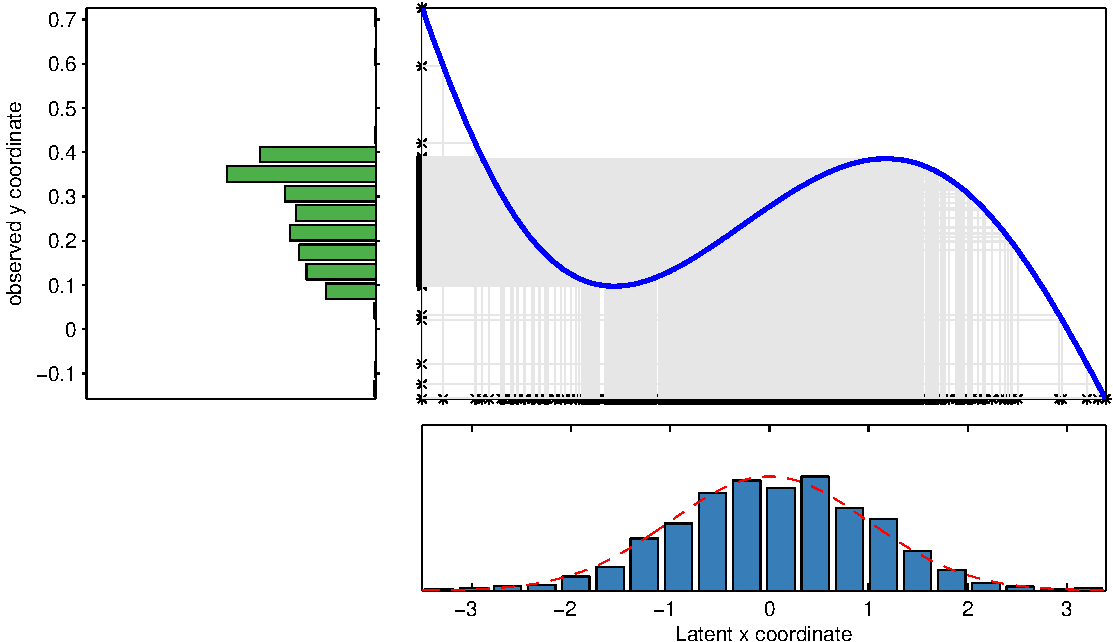
\includegraphics[width=0.8\columnwidth]{figures/gplvm_1d_draw_8} 
\caption{A draw from a Gaussian process latent variable model.  Bottom:  The latent datapoints $\vX$ are distributed according to a parametric base distribution (a Gaussian).  Top right:  A smooth function $f$ drawn from a Gaussian process prior is applied to obtain $\vY$ = $f(\vX)$.  Left:  The observed data $\vY$ is distributed according to a non-Gaussian density.}
\label{fig:gplvm_intro}
\end{figure}

The GP-LVM specifies a model wherein latent variables $\vX$ are warped by an unknown smooth, function $f$ to produce the observed data $\vY$.  The prior used over functions in the GP-LVM is the Gaussian process~\cite{rasmussen38gaussian}.

While not typically thought of as a density model, the GPLVM does define a nonparametric density over observations~\cite{nickisch2010gaussian}.   Figure \ref{fig:gplvm_intro} demonstrates how a Gaussian latent density, when warped by a random smooth function, can give rise to a non-Gaussian density in the observed space.

The dimension of the observed data ($D$) doesn't need to match the dimension of the latent space ($Q$).  When $Q$ is 2 or 3, the GP-LVM can also be used for visualization of high-dimensional data.  The mapping from $\vX$ to each dimension of the observed data is assumed to be independent, so the likelihood has a simple form which implicitly integrates over $f$:
%
\begin{align}
p(\vY | \vX,\bm{\theta})  = (2 \pi)^{-\frac{DN}{2}}  |\vK|^{-\frac{D}{2}} \exp \left( -\frac{1}{2} {\rm tr}( \vY^{\top} \vK^{-1} \vY) \right),
\label{eq:py_x}
\end{align}
where $\vK$ is the $N \times N$ covariance matrix defined 
by the kernel function $k(\vx_{n},\vx_{m})$,
and $\bm{\theta}$ is the kernel hyperparameter vector.
In this paper, we use an RBF kernel with an additive noise term:
\begin{align}
k(\vx_{n},\vx_{m}) &= \alpha \exp\left( - \frac{1}{2 \ell^2}(\vx_n - \vx_m)^{\top} (\vx_n - \vx_m) \right) + \delta_{nm} \beta^{-1}.
\end{align}




\paragraph{The density in the observed space of a deep density}

Let $\vy = \fdeep(\vx)$ be a random variable.
%
The change-of-variables formula is:
\begin{align}
p(f(\vx)) = \sum_{k=1}^{n(\vy_k = f(\vx_k))} \left| \frac{d}{dy} f^{-1}(\vy_{k}) \right| \cdot p_x(\vx_{k})
\end{align}
%
Assuming that $\fdeep(\vx)$ is one-to-one,
\begin{align}
p(f(\vx)) = p_x( \vx ) \left| \frac{  \partial f\inv(x) }{\partial x } \right|
\end{align}
%
We can use that
\begin{align}
\det(A\inv) = \frac{1}{\det(A)}
\end{align}
%
Assuming that $\fdeep(\vx)$ is one-to-one,
\begin{align}
p(f(\vx)) = p_x( \vx ) \left| J\inv(\vx) \right| = p_x( \vx ) \frac{1}{\left| J(\vx) \right|}
\end{align}

\paragraph{Eigenvalues of inverse}  We can try to prove things about the eigenvalues of $J(\vx)$.  However, in order to characterize the density of $p(\vy)$, we will need to analyse the eigenspectrum of $J\inv(\vx)$.  Helpfully, if $\lambda$ are the eigenvalues of $J$, then $\lambda \inv$ are the eigenvalues of $J\inv$.

\paragraph{Determinant in terms of Eigenvalues}  If $\lambda$ are the eigenvalues of J, then
\begin{align}
|J| = \prod_i \lambda_i
\end{align}







\section{Relation to Deep Neural Networks}

There are two reasons to think that the deep-GP prior is related to the inductive bias of deep neural networks.  First, the 

\paragraph{Weights don't change much during training}
James Martens says that the weights don't change much during training.  Perhaps we could make a plot showing the original weights versus the trained weights?

\paragraph{$L_2$ regularization of weights corresponds in a loose sense to independent Gaussian priors on the weights}
Which correspond to Gaussian processes (Neal)

